\documentclass[b5paper]{memoir}

\usepackage{fontspec}
\setmainfont
	[ Ligatures = TeX,
	Extension = .otf,
	SmallCapsFeatures={Letters=SmallCaps},
	UprightFont    = *_R,
	ItalicFont     = *_RI,
	% BoldFont       = *_B,
	BoldItalicFont = *_BI,
	]
	{LinLibertine}
\usepackage{xeCJK}
\setCJKmainfont{WenQuanYi Zen Hei Mono}

\usepackage{graphicx}
\graphicspath{ {/home/drbean/圖片/taro/} }
% \usepackage{pdf14}
\usepackage{tikz}
\usepackage{float}

\setsecnumdepth{none}
\setcounter{tocdepth}{1}

\makeatletter
\counterwithout{figure}{chapter}
\renewcommand\@memmain@floats{}
\makeatother

\begin{document}

\frontmatter

\title{\Huge An elementary guide to the 尺八 (Shakuhachi)}
\author{\huge 松本太郎 (Taro Matsumoto)}
\date{\Large 2014}
\maketitle

\cleardoublepage

\tableofcontents
\listoffigures

\cleardoublepage

\section{Preface}
This text is written as an elementary guide to the shakuhachi, the Japanese bamboo flute. Although the shakuhachi can be played by anybody who can breathe, it takes a long time to produce a sound which pleases your soul.

\par

To someone who would like to start learning shakuhachi music, I would suggest listening to many performers, and to be choosy about finding your teacher.  In this way, one can avoid the waste of time. A sword without an edge is useless. If you study under the proper teacher, the shakuhachi will be your friend for life. 

\par

I hope you experience this mystical instrument.
 
\par
                      
\hfill                                                        The Author



\cleardoublepage

\mainmatter

\section{Brief history of the instrument}
The Shakuhachi is a vertical flute made of bamboo. It was introduced from China around the 12th century. At that period, the instrument was used to play the Chinese court music called Gagaku.

\par

In medieval times, the shakuhachi became popular 
among zen monks and samurai. Many conversions were made to the instrument at this time, to make the music suitable
for Japanese sensitivity. Especially, a group of zen monks called komuso developed their compositions into a form of    
meditation called suizen (blowing zen). All these classic pieces remain today, showing the peak of the spirituality and the 
technique of shakuhachi music.

\par

After the abolition of komuso temples (1871), the shakuhachi was released from the monopoly of the komuso, and started to be used in folk music, in concert with koto and shamisen, and even in western 
music. One distinctive feature of this simple instrument is that it obtained the ability to produce all the notes
of the keyboard, already in medieval times. The basic structure has not been changed for 7~800 years, as if it is at the end of its evolution.


\section{Breath and mind}
To master the secret of shakuhachi music, your breath has to be soft and slow.
The Chinese-character word meaning “breath” consists of two different characters.
One means breath and the other one means mind.
Your breath goes fast ,when you feel sad ,angry ,or are feeling uneasy.
Your breath is not something you have tried to obtain, but was given by the Creator.
All you have to do is to let it flow freely, with no struggling or pushing.
You are not the one who controls your breath; this means that you are under the control of your breath.




\section{Meri and kari}
These two Japanese words mean bending the note down/up, by changing the position of one’s head.
Meri (メ) means to lean one’s head forward, in order to lower the note a half or whole tone. Kari (ヵ) means the opposite.

\makebox[0.5\textwidth][t]{\includegraphics[angle=90,width=0.45\textwidth]{IMG_2855.JPG}}
\makebox[0.5\textwidth][t]{\includegraphics[angle=90,width=0.45\textwidth]{IMG_2866.JPG}}



\section{Maintenance}
Thanks to its simplicity,the shakuhachi is a very durable instrument, which will last more than one thousand years, if it is stored properly. 

\par

1  Avoid sun light, and keep humidity at 55~75 per cent, to prevent cracking.\\
   Wiping the instrument with walnut/olive oil once every 3~4 months is helpful.\\
   Storing the shakuhachi in the bathroom is recommended, especially in a place like a hotel, or skyscraper, or wherever the air is deadly dry. 

\par

2  After practice, dry the inside of the instrument with a cotton cloth.

\par

3  A crack should be repaired as soon as possible, as it will grow longer and deeper.
   When it gets to the inside of the instrument, the repair work costs a lot.

\par

4  If the lacquer peels off, it should be japanned, before you play the 
   instrument again. This problem causes the worst splitting of the shakuhachi.



\section{Fingering}
\begin{figure}[H]
	\centering
	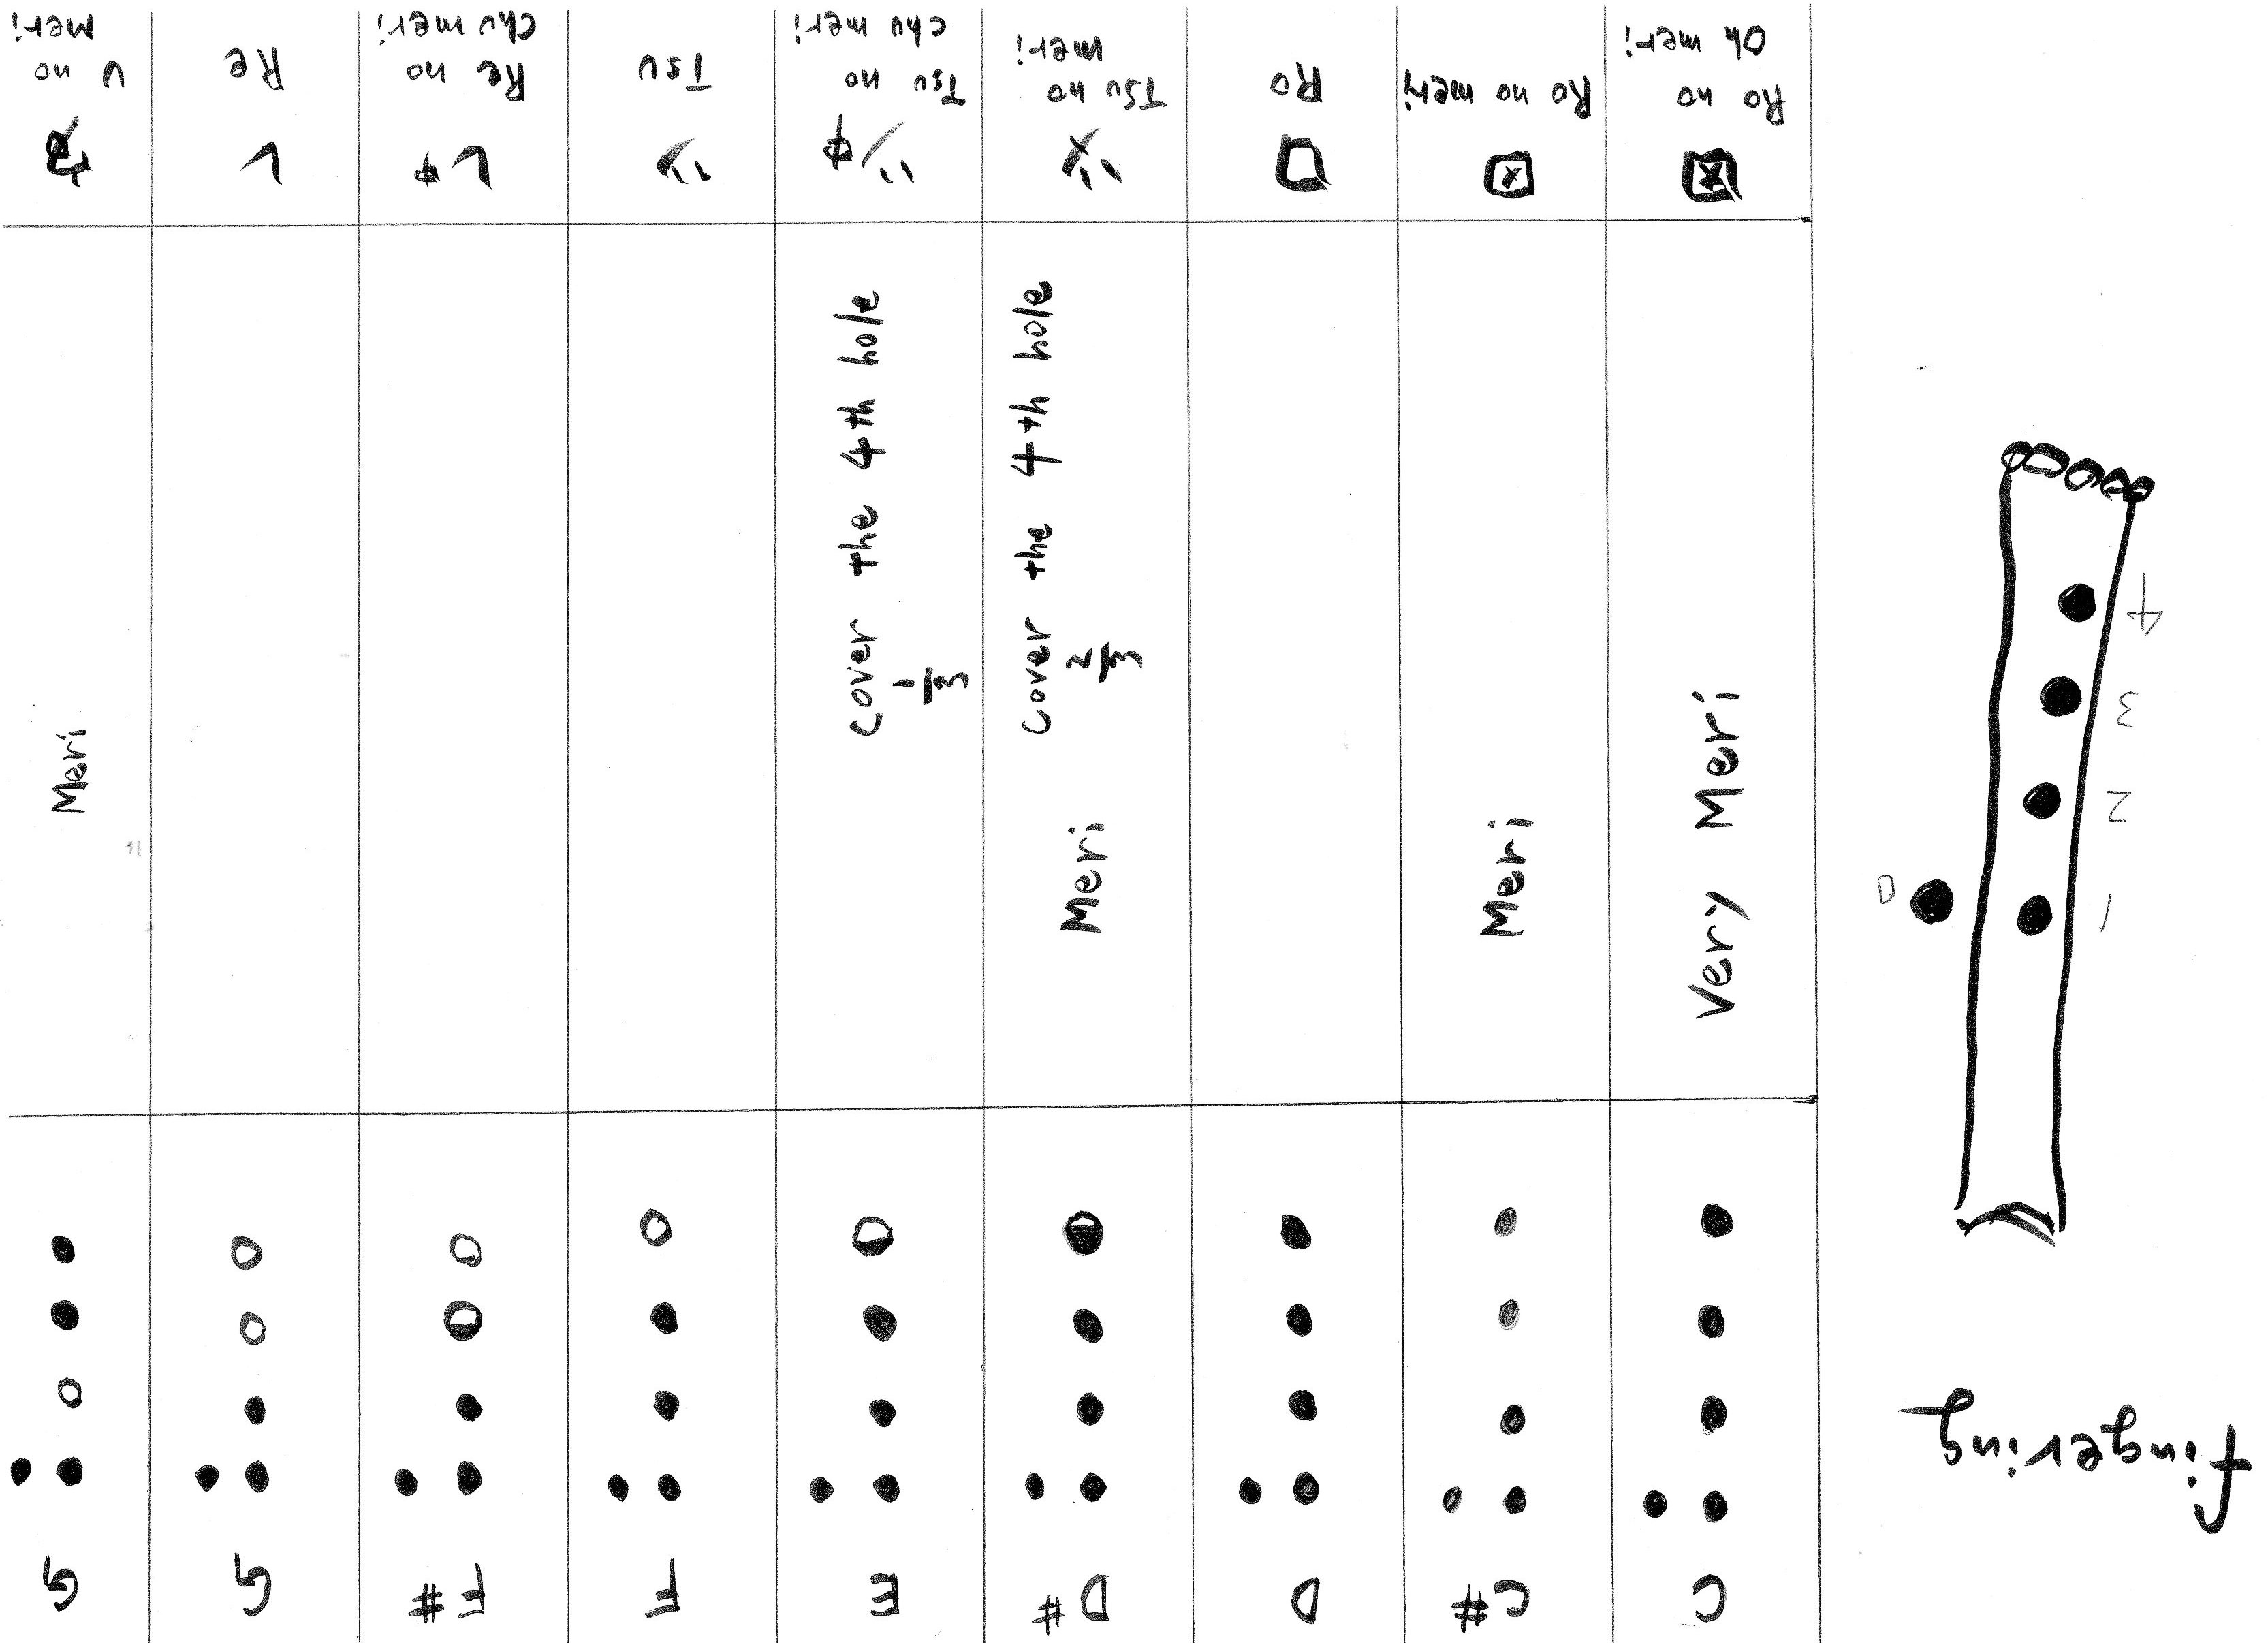
\includegraphics[angle=0,width=1.0\textwidth]{尺八の運指表1}
	\caption{Shakuhachi fingerings Part 1}
	\label{fig:shakuhachi_fingerings_1}
\end{figure}

\begin{figure}[H]
	\centering
	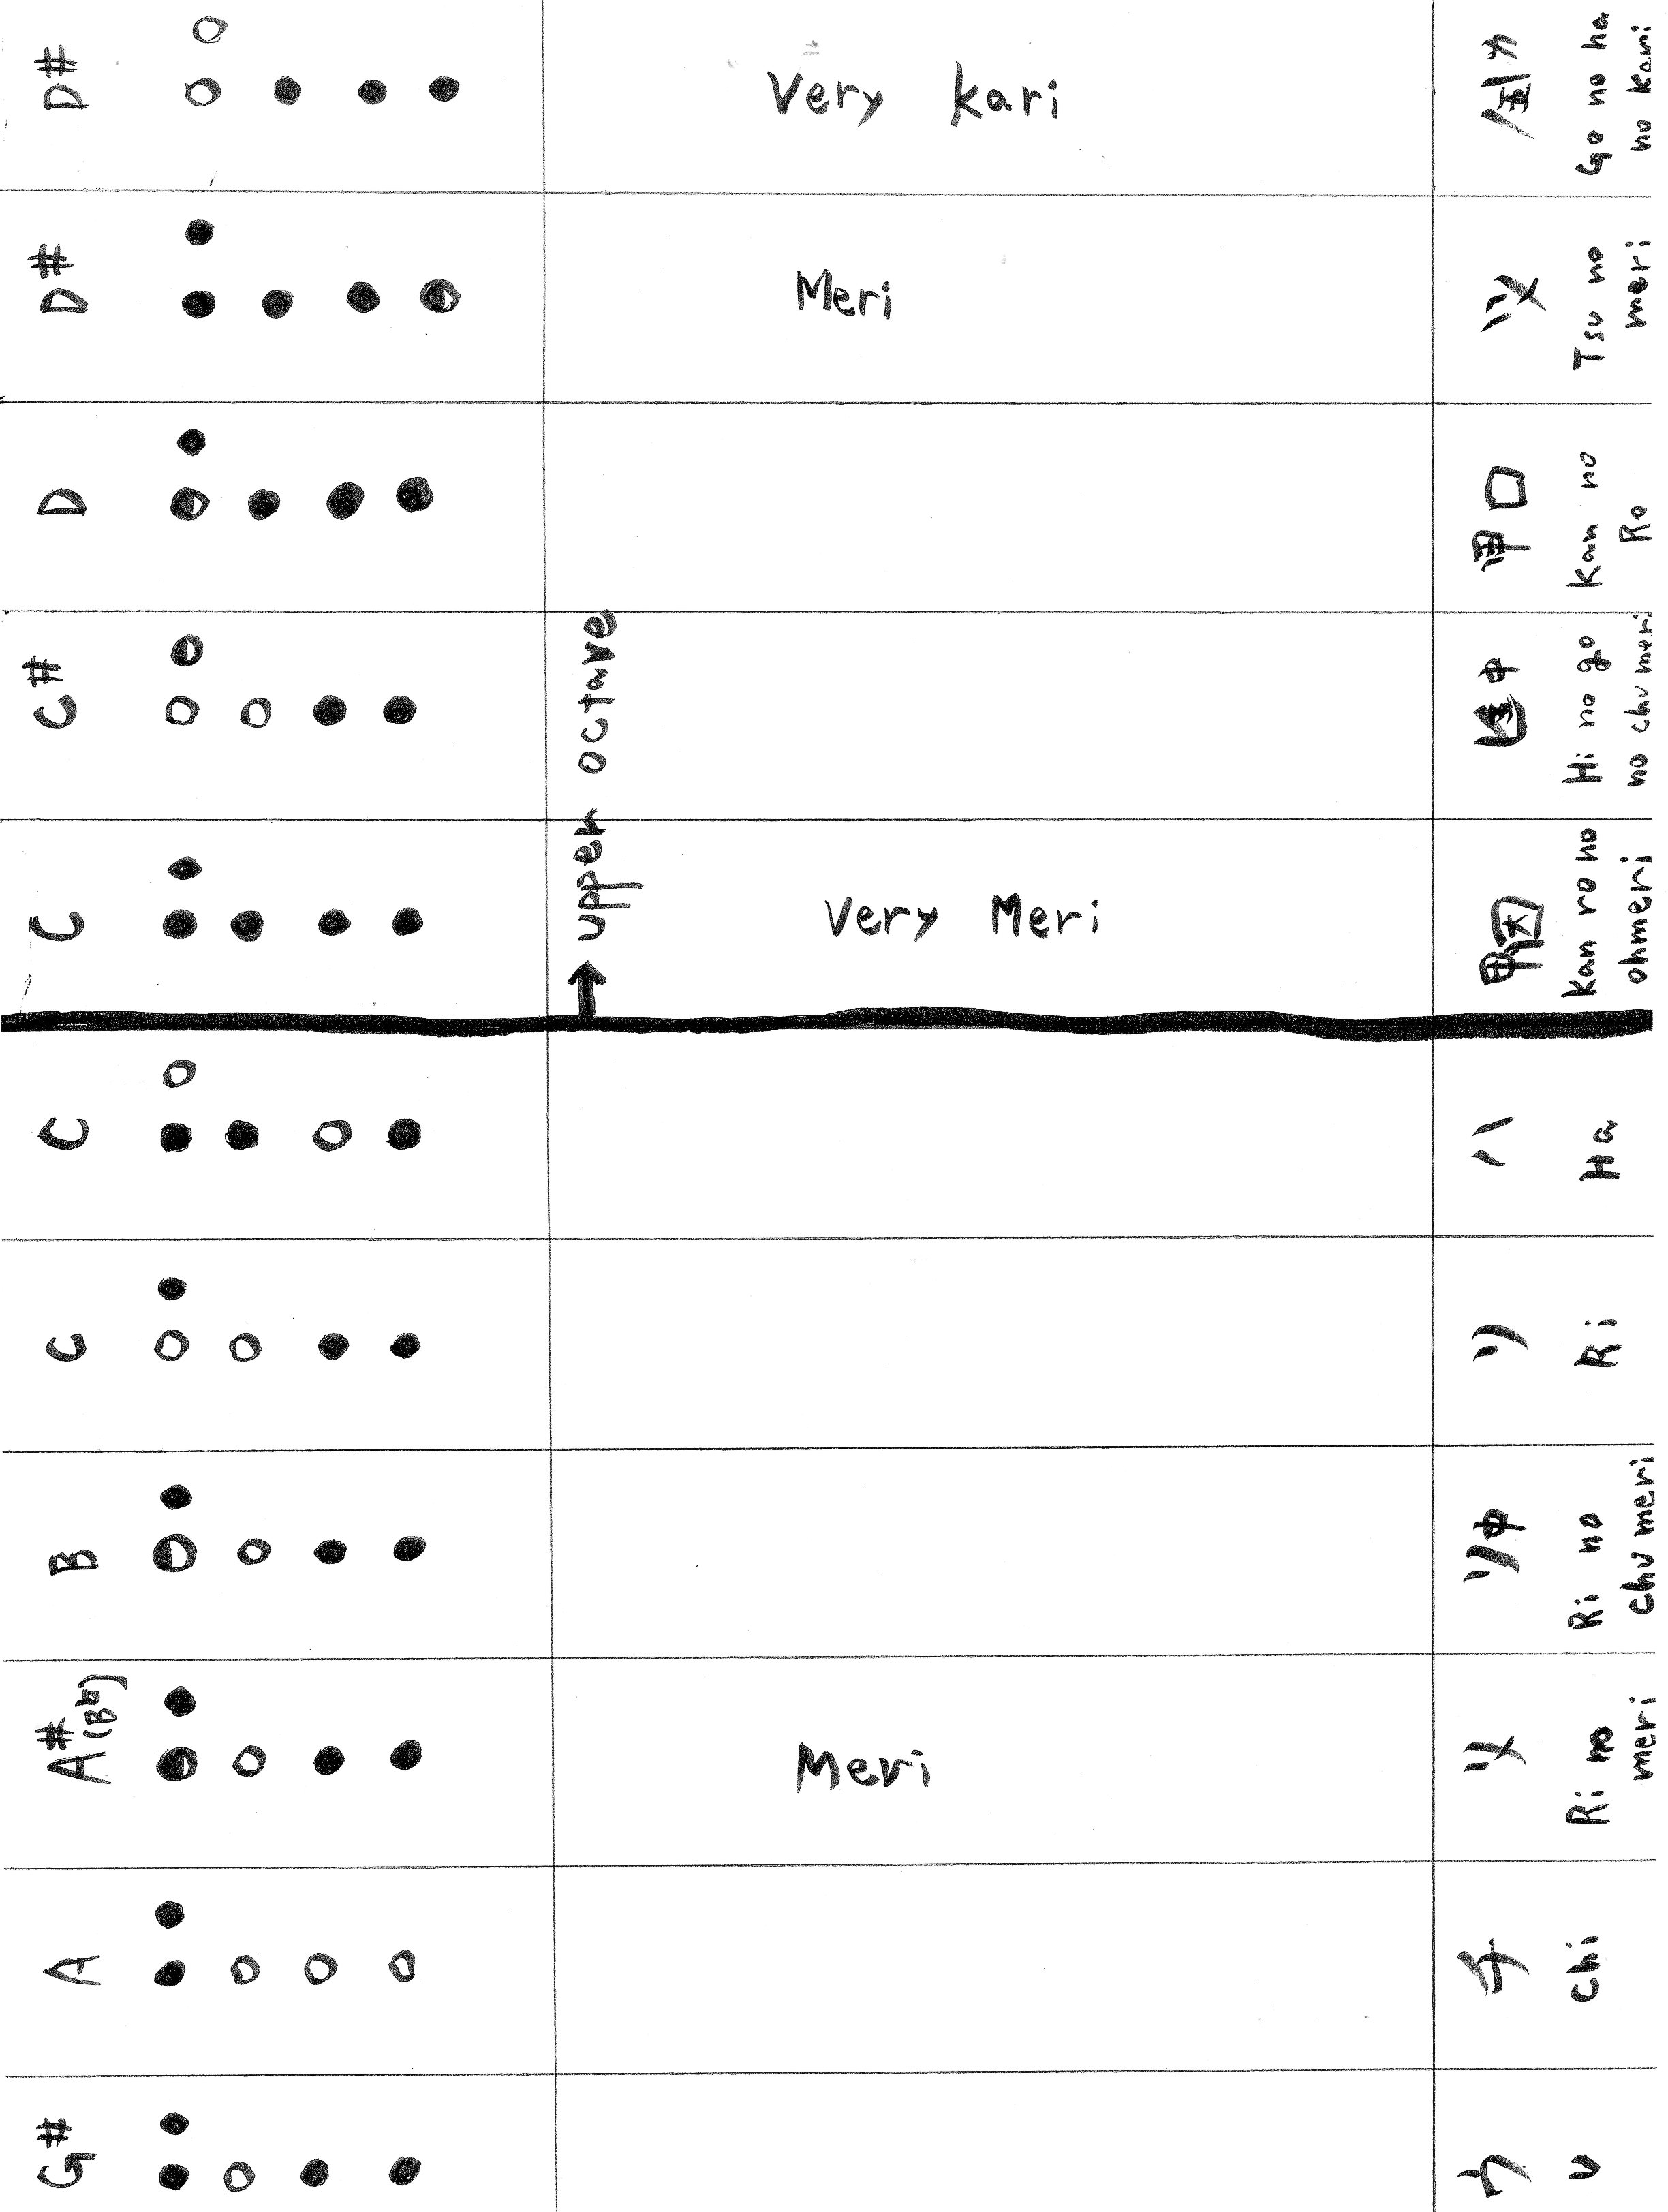
\includegraphics[angle=0,width=1.0\textwidth]{尺八の運指表2}
	\caption{Shakuhachi fingerings Part 2}
	\label{fig:shakuhachi_fingerings_2}
\end{figure}

\begin{figure}[H]
	\centering
	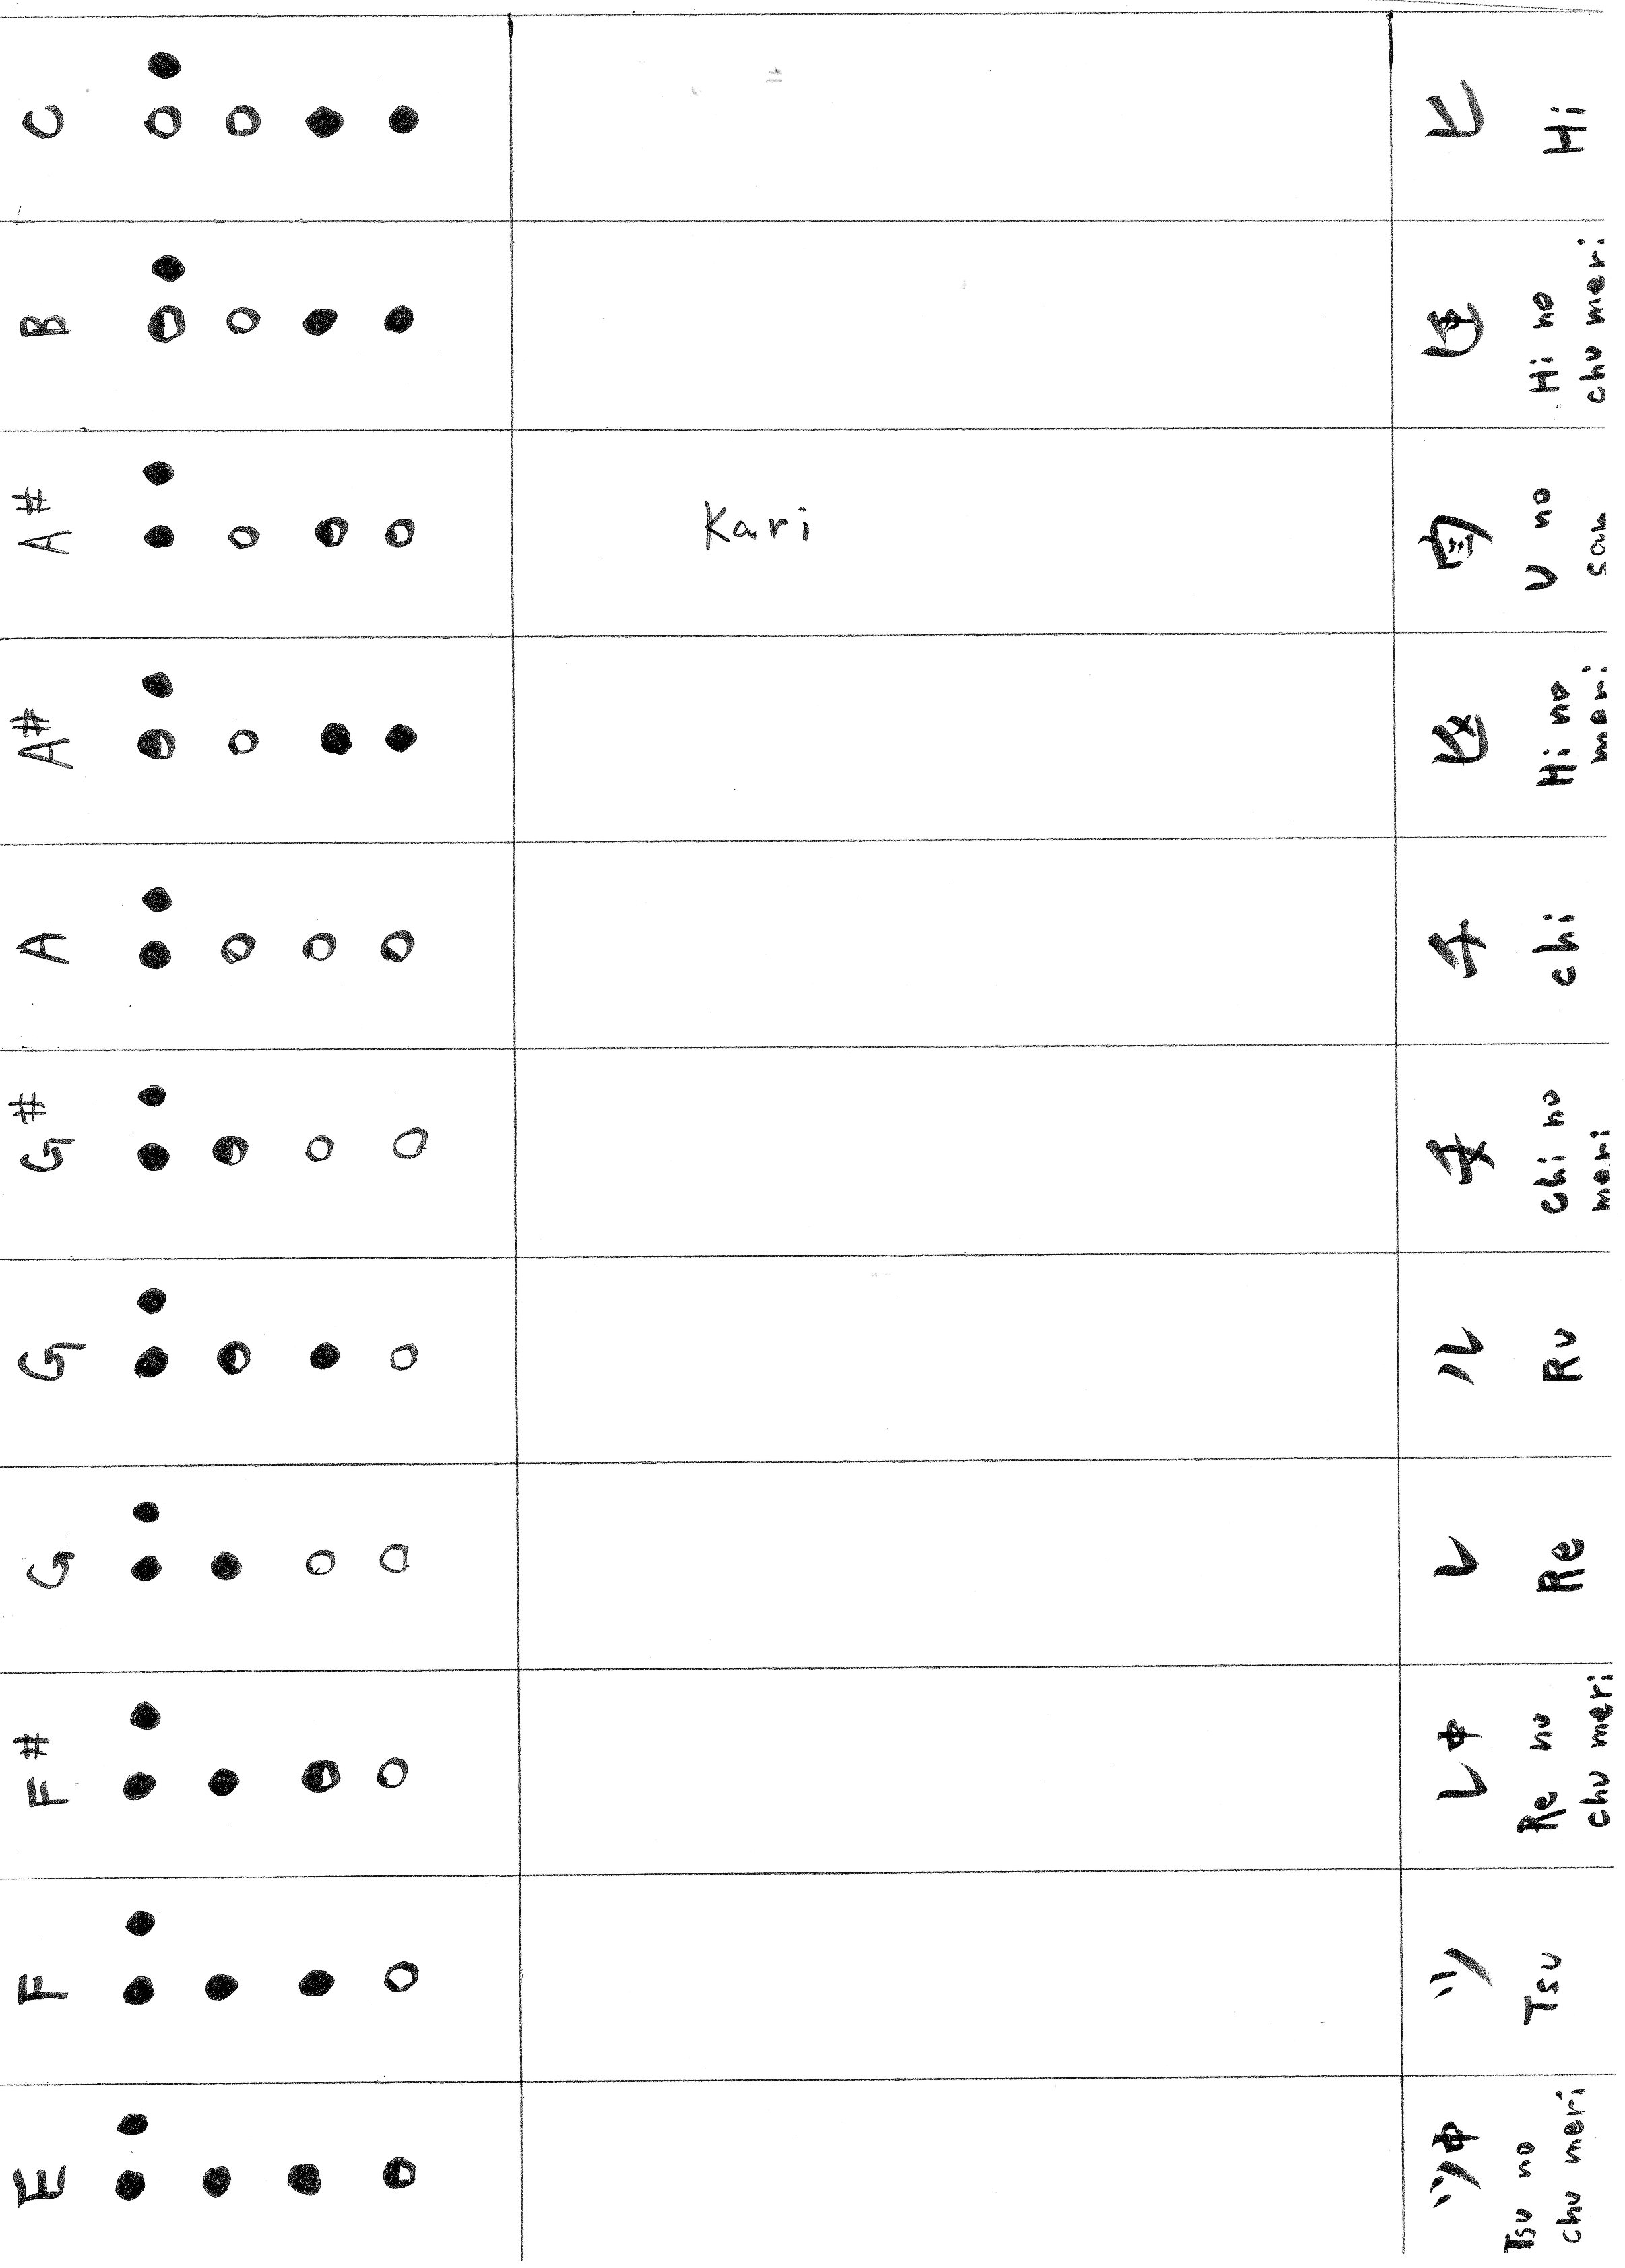
\includegraphics[angle=0,width=1.0\textwidth]{尺八の運指表3}
	\caption{Shakuhachi fingerings Part 3}
	\label{fig:shakuhachi_fingerings_3}
\end{figure}

\begin{figure}[H]
	\centering
	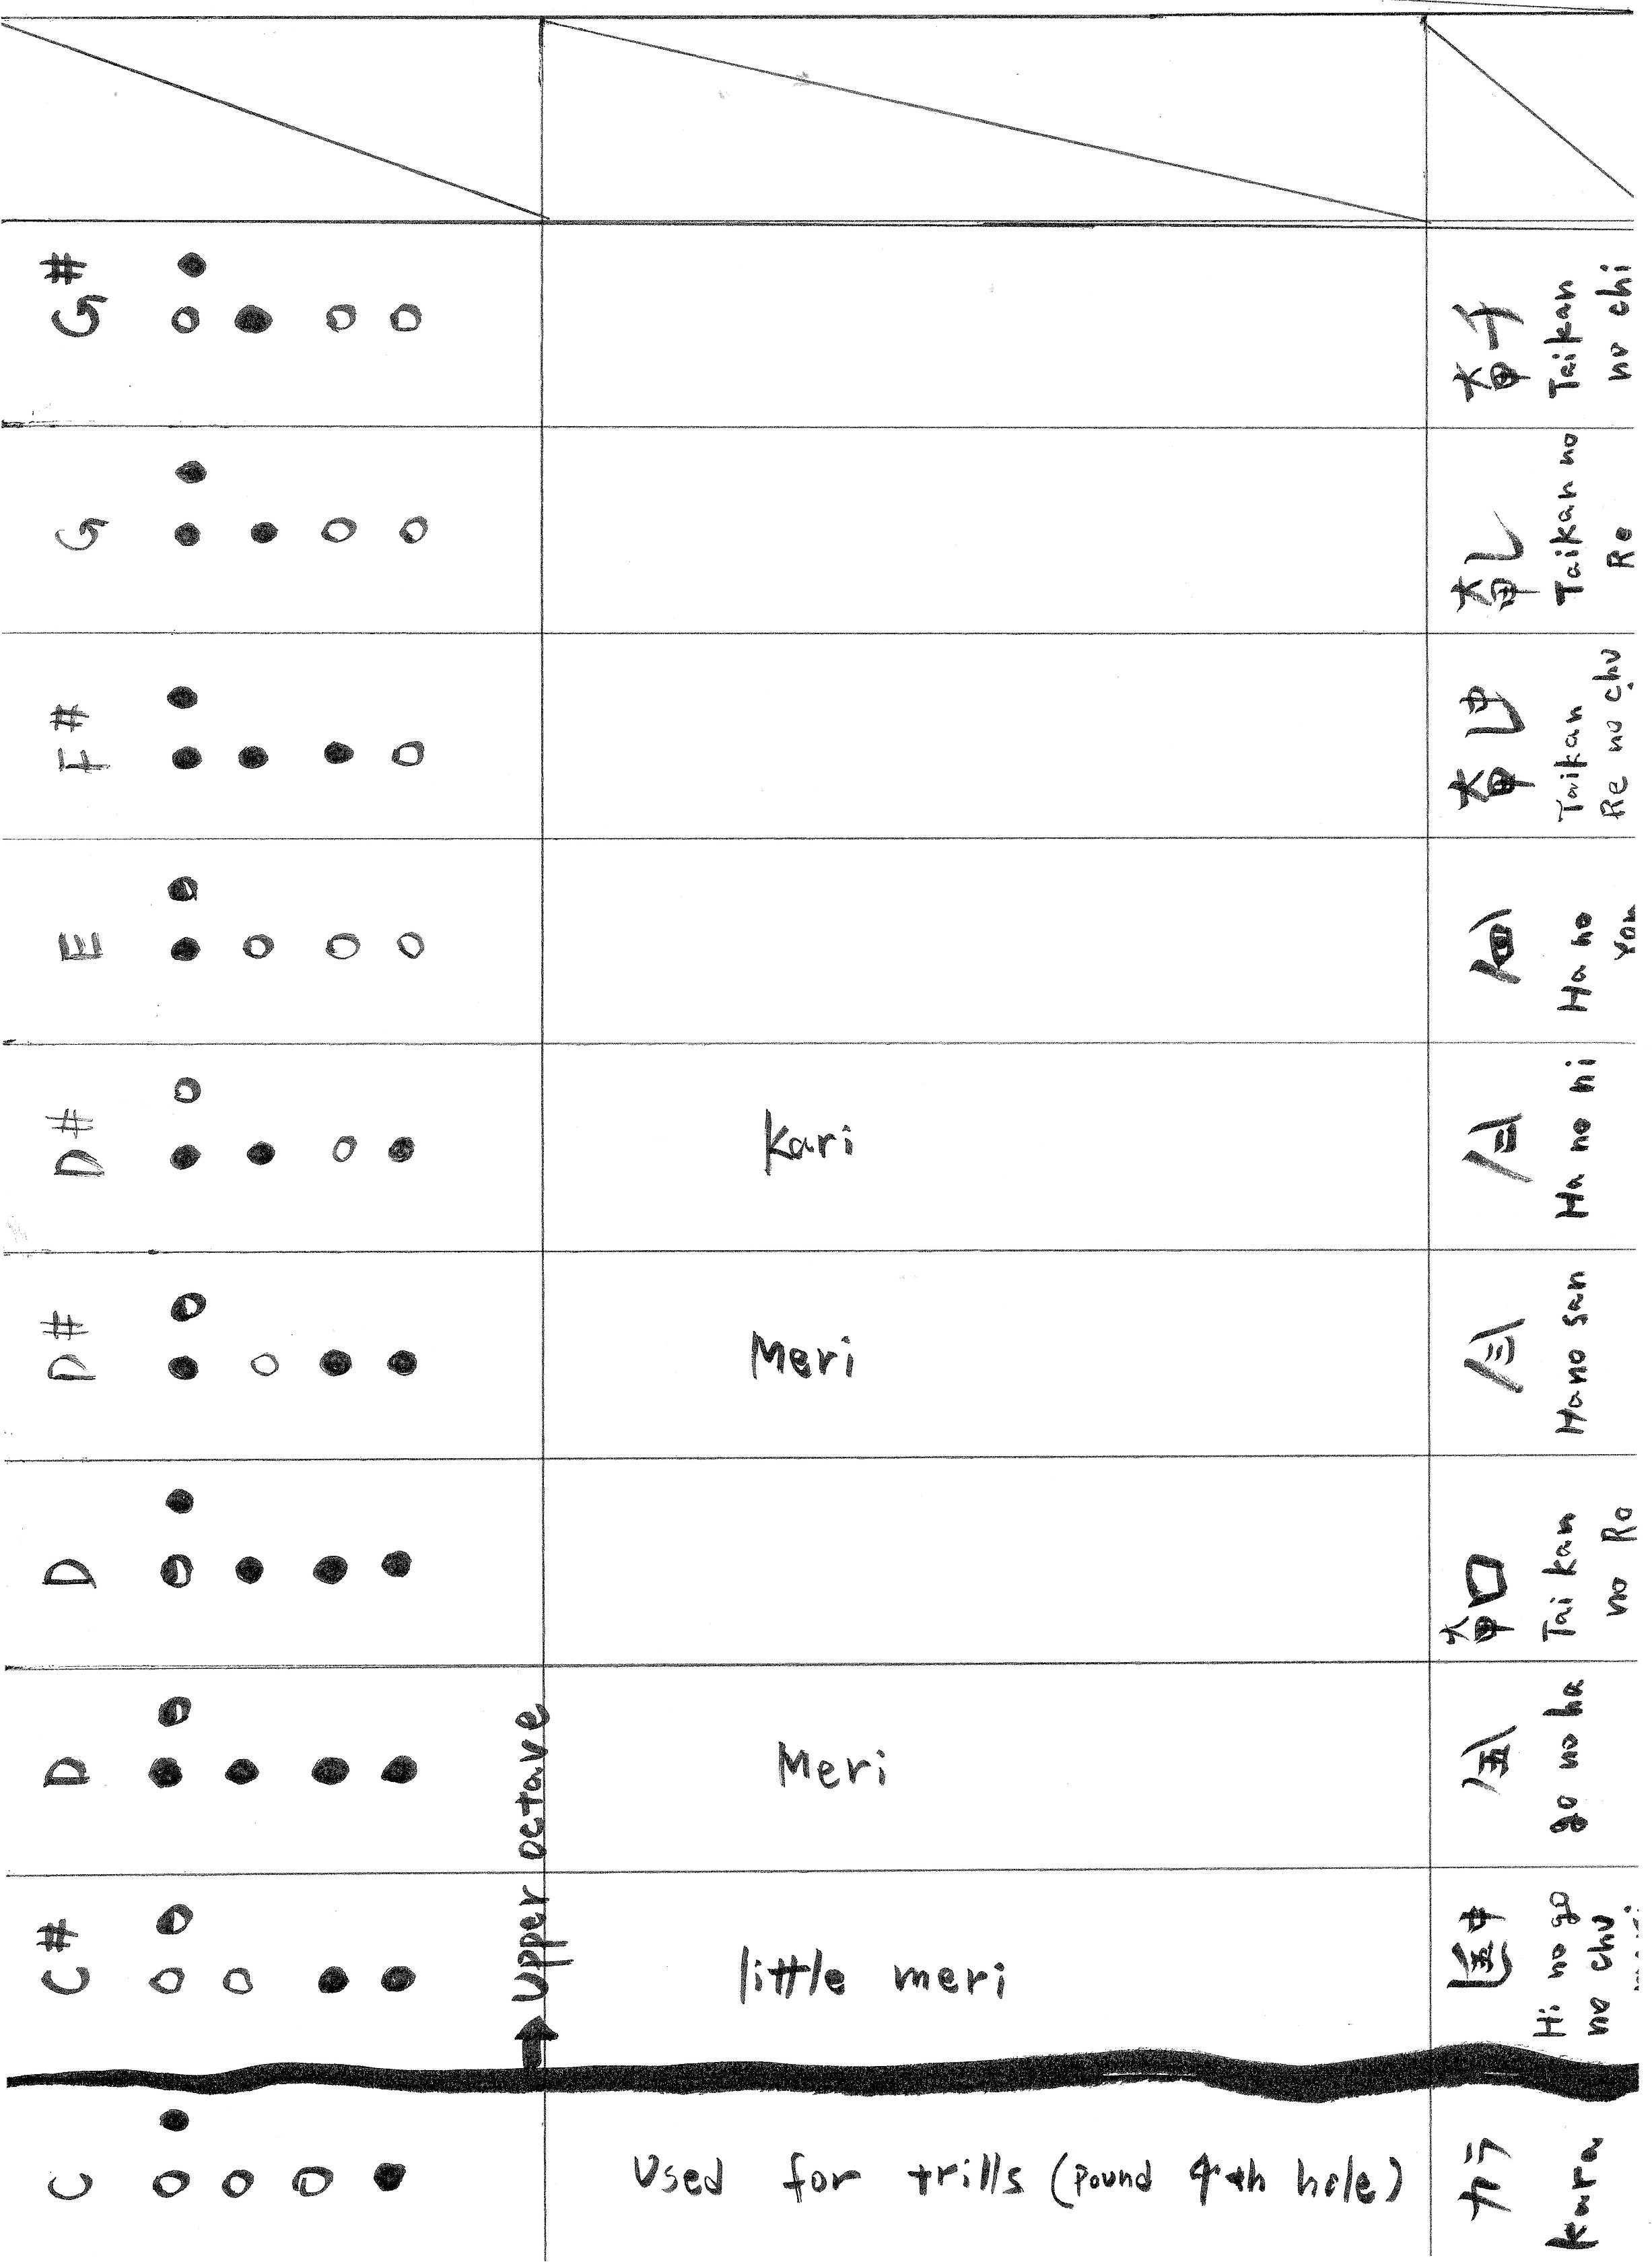
\includegraphics[angle=0,width=1.0\textwidth]{尺八の運指表4}
	\caption{Shakuhachi fingerings Part 4}
	\label{fig:shakuhachi_fingerings_4}
\end{figure}


\appendix
\appendixpage
% \addappheadtotoc

\newpage

\section{The author}
Taro Matsumoto

Born in Osaka city in 1973.
He was brought up in Nara prefecture, and spent four years studying in high school and university in Australia.
Whilst studying art history and modern thought, he accidentally came upon the the shakuhachi music of the “Watazumido school”, and decided to become a professional shakuhachi player. The music of Watazumido is based on the classic pieces composed by anonymous Zen monks of medieval times. The creator of Watazumido revitalized this classic music with superior technique and the precise logic of breath training. These compositions adopt the representative components of  Japanese spirituality, such as zen, Buddhist chant, native Japanese music and the sounds heard in the natural environment. Matsumoto has studied under Riley Lee, Toshimitsu Ishikawa, and Reishou Yonemura. 

Following are the forms of music Matsumoto has been playing. 

Watazumido honkyoku   classic pieces derived from the 12th century

Kinko ryu honkyoku      classic pieces of the Kinko school

San Kyoku               ensembles with koto and shamisen

He supplies the music for plays and operas,and also is an excellent improviser.


                                         end        


\backmatter

\end{document}

